\section{Velocity Analysis}\label{sec:velocityAnalysis}
We have held multiple sessions of Planning Poker during the project, as seen in e.g. \ref{sec:sprintPlanningSprint3}.

Doing so has allowed us to understand the velocity we work at over time. To recap: \textit{Velocity is measured by taking the sum of the estimates of each completed task in a sprint\cite{sutherlandScrumArtDoing2014}.}

Once you have your velocity over multiple sprints, you can begin tracking and analyzing how the velocity changes over time. This can be useful to measure how experiments or changes to processes affect the team's velocity.

Burndown charts can be a useful method of visualizing project or sprint progress over time. In essence, they measure the amount of work left, in relation to the amount of work that has been completed. They are especially useful in Scrum and Agile projects\cite{HowCreateBurndown2021}. We will, however, not create such charts for our project. One reason is a lack of data, as we did not create estimates until sprint 3.
In addition, we shortened the sprints to a duration of two weeks each, which would have given us 4 work-days per sprint. Creating a sprint burndown chart over such a short duration would have cost more than it would have been worth.
Likewise, creating a product burndown chart for our layer would have been almost impossible, as there did not, at most times, exist a product backlog to measure against.

Instead, we have opted to sum the estimates of each task in a sprint, and then use this to calculate the velocity for the sprint. We used that estimate to measure against when selecting tasks in the following sprints, trying to achieve the same or better velocity. The data for this can be seen in figure \ref{img:velocityOverTime}.

\begin{figure}[h!]
\centering
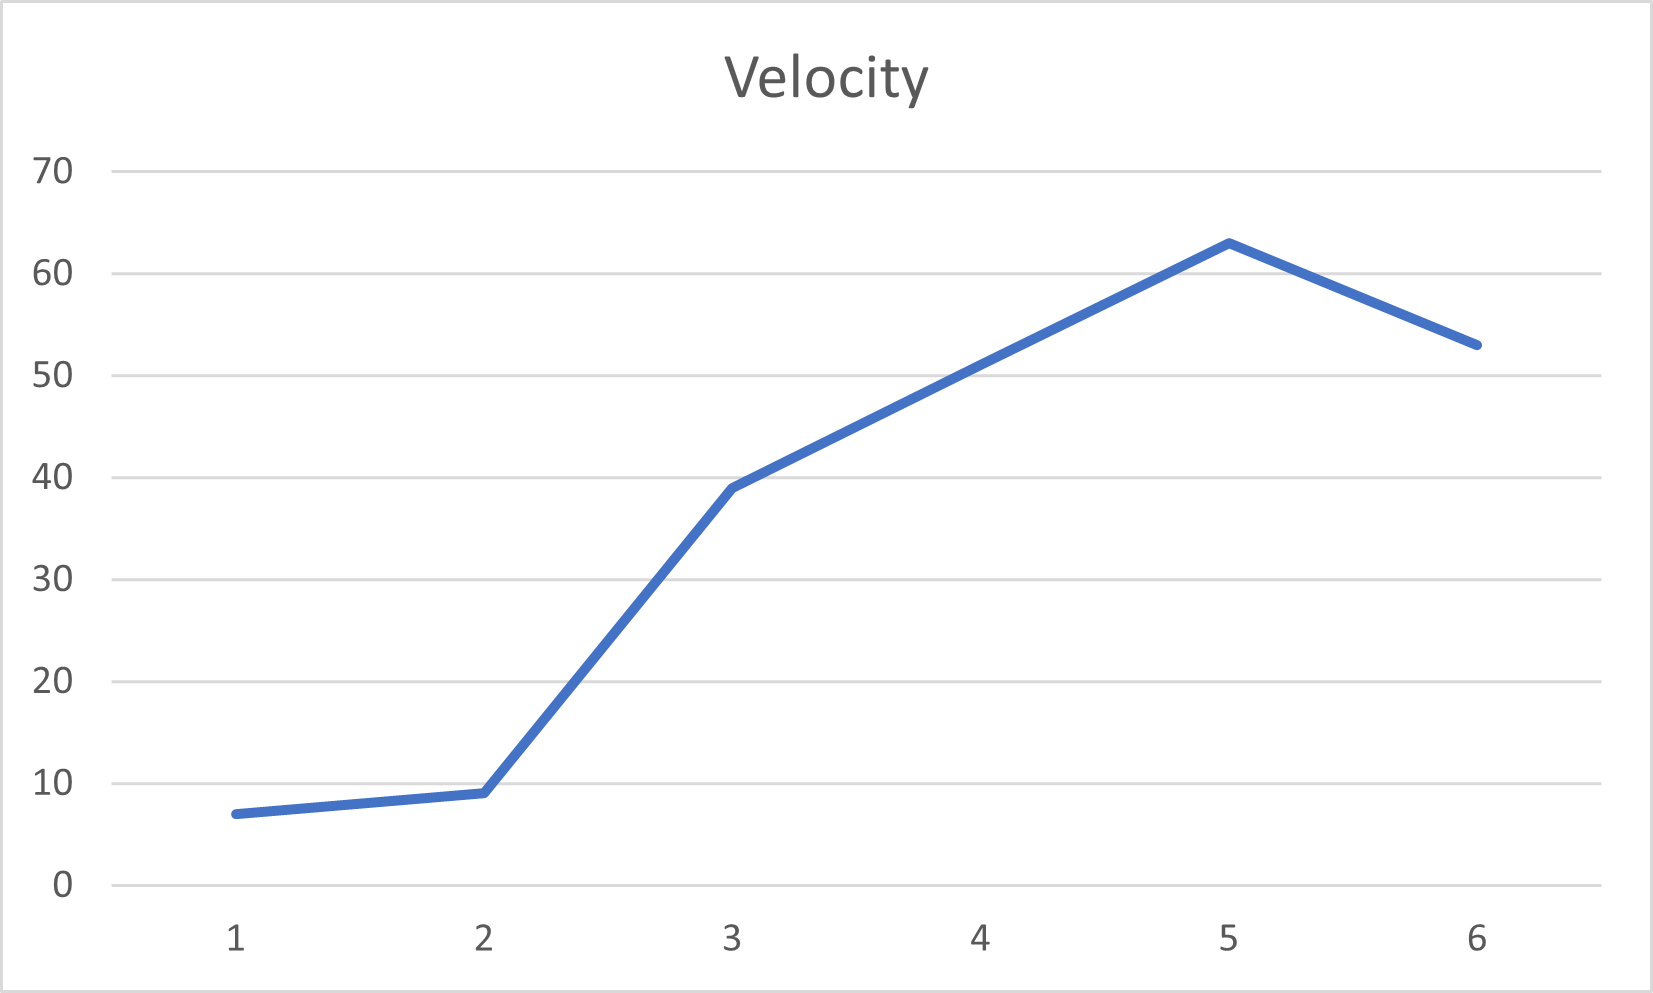
\includegraphics[width=0.8\textwidth]{Images/VelocityAnalysis.png}
\caption{Velocity over time}
\label{img:velocityOverTime}
\end{figure}

As can be seen in figure \ref{img:velocityOverTime}, the velocity of the project has increased over time.
There can be many possible explanations for this, but we believe it to be the product of a continuous improvement process.
After most sprints, we have reflected upon our process and attempted to improve it in the following sprint.

Notably, we had a low velocity in the first two sprints. This is, in no small part, due to a lack of planning and organization. In the following sprints, we improved our process, and gained a much higher velocity because of it.
This is especially clear when we, from sprint 4, changed the sprint duration to a duration of two weeks, yet we became much faster than we had been before.
A possible explanation is that we, from sprint 3, got stricter in our granularization and specification of tasks, which created less ambiguity while working.
That sprint seems to have been the turning point in our process and approach. Because in that same sprint, we changed our planning poker strategy, changed how we acquired user stories, and made other process improvements, which seem to have been beneficial --- as can be seen in the figure.

One of our bigger takeaways was learned in sprint 4, where we found that we had to be careful to fix issues as they occur. The longer an issue remains unsolved, the more expensive it becomes to resolve it.

In sprint 6, our velocity decreased by about ten points. This seems like a step back --- and it is --- but we learned something valuable from it.
First, during the sprint, we removed tasks from the sprint, as we realized that they were not needed. 
Secondly, we worked on tasks during the sprint which required collaboration and communication with other teams. This caused multiple delays, as we had to wait for other teams to either respond, or to finish their work. Therefore, in the future, we believe that we should both assign more points to such tasks, but should also be careful not to spend too much time waiting, and instead shift focus while waiting for the other teams. Of course, it is not possible to spend all waiting time on another task, as we had to actively respond to their queries during that time as well.

In general, we are very satisfied with our improvements throughout the project. Our process and approach has improved, and we have learned from our experiences. More importantly, we managed to rapidly put what we learned to use, and fix impediments quickly.

% Sprint 3 retrospective: remove the todo after finishing here. Refer to this chapter, perhaps.